% DefensePresentation.tex — ProjectV защита 2026-06-17
% Компиляция: xelatex (через latexmk -pdfxe)
% Источник verbatim: docs/DefenseScript_Team.md
% Структура: docs/DefensePresentation_Structure.md

% header.tex — общий preamble для DefensePresentation.tex
% Компилируется через XeLaTeX (xelatex + latexmk -pdfxe)
% Тема: Madrid (по умолчанию Beamer), шрифты Liberation (Cyrillic полная поддержка)

\documentclass[11pt,aspectratio=169]{beamer}

% --- Кодировка и язык ---
\usepackage{fontspec}
\usepackage{polyglossia}
\setmainlanguage{russian}
\setotherlanguage{english}
\setmainfont{Liberation Sans}
\setsansfont{Liberation Sans}
\setmonofont{Liberation Mono}

% --- Beamer theme: Madrid (сине-серый корпоративный стиль) ---
\usetheme{Madrid}
\usecolortheme{default}
% Цветовая схема: тёмно-синий заголовок, серый фон
\definecolor{projectvblue}{RGB}{30, 60, 110}
\definecolor{projectvgray}{RGB}{200, 200, 210}
\setbeamercolor{frametitle}{bg=projectvblue,fg=white}
\setbeamercolor{framesubtitle}{bg=projectvblue,fg=white}
\setbeamercolor{block title}{bg=projectvblue,fg=white}
\setbeamercolor{block body}{bg=projectvgray,fg=black}
\setbeamercolor{title}{bg=projectvblue,fg=white}

% --- Математика, таблицы, графика, спецсимволы ---
\usepackage{amsmath}
\usepackage{amssymb}
\usepackage{booktabs}
\usepackage{array}
\usepackage{multirow}
\usepackage{colortbl}
\usepackage{xcolor}
\usepackage{graphicx}
\usepackage{url}
\usepackage{hyperref}
\hypersetup{colorlinks=true,urlcolor=projectvblue}

% --- QR-код (для титульного слайда) ---
\usepackage{qrcode}

% --- Убрать навигационные символы Beamer (для чистого PDF) ---
\setbeamertemplate{navigation symbols}{}
% Скрыть нижнюю панель с названием секции
\setbeamertemplate{footline}{}
% Показывать только номер слайда в футере
\setbeamertemplate{footline}[frame number]

% --- Утилиты ---
\newcommand{\code}[1]{\texttt{\small #1}}
\newcommand{\filament}[1]{\textit{#1}}

% Подавить предупреждения о hyperref / Beamer
\RequirePackage{silence}
\WarningFilter{latex}{You have requested}

% --- Каталоги для графики ---
\graphicspath{{./}{./screenshots/}}

% --- Метаданные PDF ---
\title{ProjectV}
\subtitle{Открытый высокопроизводительный воксельный движок}
\author{Команда <<Черепашки Ninja>>}
\institute{МФТИ-1-2024}
\date{2026-06-17}


\begin{document}

% === Слайд 1: Титульный слайд (без ссылок на репозиторий, с описанием сборки) ===
\begin{frame}[plain]
  \titlepage
  \vspace{0.8em}
  \begin{center}
    \scriptsize\textcolor{projectvblue}{\textbf{Окружение сборки:}}
    CMake 3.30+ $\bullet$ Clang 22 (C++26) $\bullet$ Vulkan SDK 1.4.350
  \end{center}
\end{frame}

% === Слайд 2: Проблема и ценность ===
\begin{frame}{Проблема: Отсутствие открытого низкоуровневого базиса}
  \framesubtitle{Для кого и почему это важно}
  \begin{columns}[T]
    \begin{column}{0.48\textwidth}
      \textbf{Целевая аудитория и контекст:}
      \begin{itemize}
        \item Разработчики воксельных инди-игр.
        \item Исследователи компьютерной графики.
        \item Студенты профильных IT-специальностей.
      \end{itemize}
    \end{column}
    \begin{column}{0.48\textwidth}
      \textbf{Существующие ограничения:}
      \begin{itemize}
        \item \filament{Закрытость:} Исходный код коммерческих движков (Minecraft) недоступен.
        \item \filament{Абстракция:} Универсальные движки (Unity/Godot) скрывают прямой контроль GPU.
        \item \filament{Устаревание:} Альтернативы используют OpenGL без DOD-структур.
      \end{itemize}
    \end{column}
  \end{columns}
  \vspace{1em}
  \begin{center}
    \textbf{Ценность проекта:} Предоставление разработчику полного контроля над памятью и ресурсами видеокарты.
  \end{center}
\end{frame}

% === Слайд 3: Цели и спецификации (исправлено выпирание таблицы) ===
\begin{frame}{Цели проекта и требования ТЗ}
  \framesubtitle{Ход реализации и численные критерии верификации}
  \begin{center}
    \textbf{Статус выполнения ТЗ: 38 требований закрыто $\bullet$ 5 отложено $\bullet$ 0 критических сбоев}
  \end{center}
  \vspace{0.5em}
  \small
  \begin{table}
    \centering
    \resizebox{\textwidth}{!}{%
      \begin{tabular}{lll}
        \toprule
        \textbf{Критерий успеха} & \textbf{Целевой показатель} & \textbf{Метод верификации} \\
        \midrule
        Кадровая частота & 500+ FPS (сцена VoxelLab, Debug) & Встроенный HUD-счетчик \\
        Размер исполняемого файла & 19 МБ (Release, сжатие $-73\%$) & Физический размер ELF \\
        Тесты ядра системы & 14 из 14 тестов успешно пройдены & Конвейер CTest \\
        Визуальная корректность & 6 из 6 графических слоев верны & Скрипты Runtime Smoke \\
        Предупреждения компилятора & 0 предупреждений в нашем коде & Сборка Clang 22 с -Wall \\
        \bottomrule
      \end{tabular}%
    }
  \end{table}
\end{frame}

% === Слайд 4: Демонстрация прототипа VoxelLab ===
\begin{frame}{Прототип: Тестовая лаборатория VoxelLab}
  \framesubtitle{Демонстрация работы ключевых систем рендеринга и симуляции}
  \begin{center}
    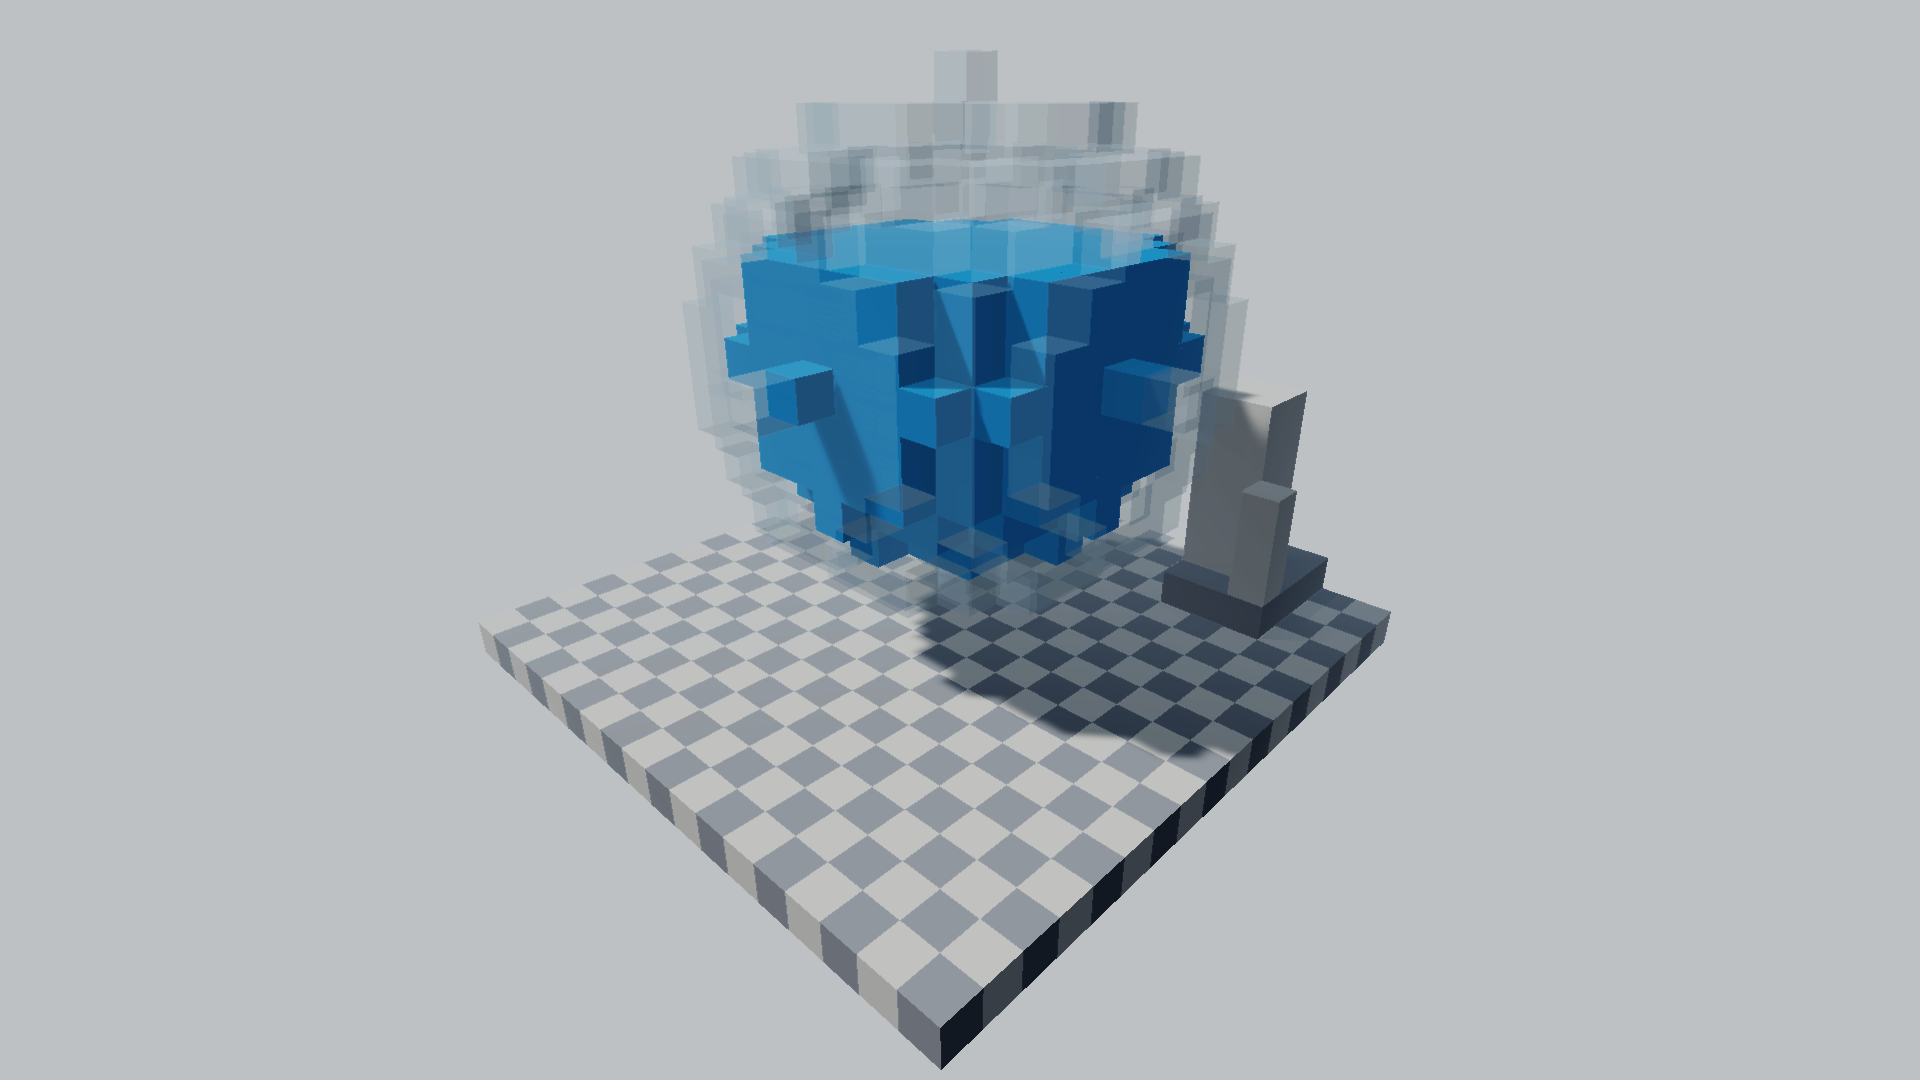
\includegraphics[width=0.45\textwidth]{screenshots/voxel_lab.png}
  \end{center}
  \vspace{-0.3em}
  \scriptsize
  \begin{columns}[T]
    \begin{column}{0.32\textwidth}
      \textbf{Физические свойства материалов:}
      \begin{itemize}
        \item \filament{Стекло (Glass):} твердое, прозрачное, не отбрасывает каскадную тень.
        \item \filament{Жидкость (Fluid):} текучая, полупрозрачная, отбрасывает тень.
      \end{itemize}
    \end{column}
    \begin{column}{0.32\textwidth}
      \textbf{Счетчик производительности:}
      \begin{itemize}
        \item Уверенное удержание 500+ FPS на сцене из 27 чанков в отладочной конфигурации.
      \end{itemize}
    \end{column}
    \begin{column}{0.32\textwidth}
      \textbf{Оптимизация геометрии:}
      \begin{itemize}
        \item Жадный мешинг объединяет смежные стороны вокселей одного типа в крупные квады.
      \end{itemize}
    \end{column}
  \end{columns}
\end{frame}

% === Слайд 5: Анализ аналогов и ниша проекта (исправлено выпирание таблицы) ===
\begin{frame}{Сравнение с существующими решениями}
  \framesubtitle{Ниша и архитектурные отличия ProjectV}
  \scriptsize
  \begin{table}
    \centering
    \resizebox{\textwidth}{!}{%
      \begin{tabular}{lccccc}
        \toprule
        \textbf{Движок / Проект} & \textbf{Стек} & \textbf{API} & \textbf{DOD} & \textbf{Шейдерный мешинг} & \textbf{Лицензия} \\
        \midrule
        Minecraft Java & Java & OpenGL $\to$ Vulkan & Нет & Нет & Коммерческая \\
        Minetest & C++17, Lua & OpenGL & Нет & Нет & LGPL 2.1 \\
        VoxelCore & C++17 & OpenGL & Нет & Нет & MIT \\
        Veloren & Rust & wgpu (Vulkan) & ECS & Частично & GPL 3.0 / MIT \\
        \rowcolor{projectvgray}
        \textbf{ProjectV (наш)} & \textbf{C++26} & \textbf{Vulkan 1.4} & \textbf{Да (SoA)} & \textbf{Да (Compute)} & \textbf{MIT} \\
        \bottomrule
      \end{tabular}%
    }
  \end{table}
  \normalsize
  \vspace{0.5em}
  \textbf{Ключевой технологический пробел:} \\
  Ни один открытый воксельный движок на рынке не предоставляет готовый низкоуровневый базис,
  сочетающий стандарт C++26, Vulkan 1.4 и Data-Oriented Design.
\end{frame}

% === Слайд 6: Архитектурные принципы и DOD ===
\begin{frame}{Архитектура и Data-Oriented Design}
  \framesubtitle{Распределение обязанностей и компоновка памяти}
  \begin{center}
    \code{SDL3 Main Loop} $\to$ \code{AppState (PIMPL)} \\[0.3em]
    $\big\downarrow$ \\[0.3em]
    \begin{tabular}{ccc}
      \code{Renderer (Vulkan 1.4)} & \code{Physics (Jolt)} & \code{ECS (Flecs)}
    \end{tabular}
  \end{center}
  \vspace{1em}
  \textbf{Физика Data-Oriented Design (DOD):}
  \begin{itemize}
    \item \textbf{Чанки $8\times8\times8$:} Размер структуры чанка равен 32 байтам ($2$ SSE-регистра).
          Полностью исключает промахи кэша L1 (объем 32 КБ на архитектуре Zen 3).
    \item \textbf{Компоновка вокселей:} Хранение материалов в плоском непрерывном векторе
          \code{std::vector<uint8\_t>} внутри общего контекста \code{VoxelWorld}.
    \item \textbf{Связь с ECS:} Мир Flecs работает как пассивное read-only зеркало данных
          \code{VoxelWorld} без накладных расходов на владение.
  \end{itemize}
\end{frame}

% === Слайд 7: GPU-мешинг и симуляция жидкостей ===
\begin{frame}{Реализация систем воксельного мира}
  \framesubtitle{Алгоритм жадного мешинга и клеточный автомат воды}
  \begin{columns}[T]
    \begin{column}{0.48\textwidth}
      \textbf{Жадный мешинг на GPU:}
      \begin{itemize}
        \item \filament{Алгоритм Лысенкова:} Реализован в compute-шейдере \code{voxel\_mesh.comp}.
        \item \filament{Логика:} 6 поочередных проходов по осям ($\pm X, \pm Y, \pm Z$).
        \item \filament{Эффективность:} Объединение смежных граней одного типа снижает число
              полигонов и вызовов отрисовки на $30{-}50\%$.
      \end{itemize}
    \end{column}
    \begin{column}{0.48\textwidth}
      \textbf{Клеточный автомат жидкостей:}
      \begin{itemize}
        \item \filament{Двойная буферизация:} Чтение из снимка состояния, запись --- в буфер
              \code{next[]}. Устраняет баги наложения.
        \item \filament{Правила:} Гравитационное падение (\code{f\_fall}) и распределение
              (\code{f\_spread}) на частоте 20 Гц.
        \item \filament{Рандомизация:} Пространственное Teschner-хэширование для воспроизводимости потоков.
      \end{itemize}
    \end{column}
  \end{columns}
\end{frame}

% === Слайд 8: Верификация и автоматическое тестирование ===
\begin{frame}{Верификация и автоматическое тестирование}
  \framesubtitle{Тестирование логики ядра и графического конвейера}
  \begin{block}{14 наборов автоматических тестов ядра (CTest)}
    \small
    Покрытие критического кода: математика, инвалидация грязных чанков, walk-контроллер,
    жадный мешинг, клеточный автомат воды, отсечение по фрустуму.
    \begin{center}
      \textbf{Результат: 14/14 успешно пройдены} (0.78 с в Debug / 0.06 с в Release)
    \end{center}
  \end{block}

  \begin{block}{Автоматические визуальные Smoke-тесты}
    \small
    Запуск приложения в фиксированной точке сцены VoxelLab с поканальным анализом рендеринга.
    \begin{center}
      Сравнение пиксель-в-пиксель: \textbf{6 из 6 проходов успешны}
    \end{center}
    \scriptsize
    \begin{tabular}{cccccc}
      \textbf{FINAL} & \textbf{SHDW} & \textbf{CSM} & \textbf{CTSH} & \textbf{AOCC} & \textbf{LOCL} \\
      Финальный кадр & Тени каскадов & Слои каскадов & Контактные тени & Фоновое затенение & Точечный свет \\
    \end{tabular}
  \end{block}
\end{frame}

% === Слайд 9: Дополнительные функциональные возможности ===
\begin{frame}{Дополнительные функциональные возможности}
  \framesubtitle{Ассет-пайплайн, аудиоподсистема, сохранение мира и отладка}
  \begin{columns}[T]
    \begin{column}{0.48\textwidth}
      \textbf{Загрузка полигональных моделей:}
      \begin{itemize}
        \item Использование парсера \code{fastgltf} для glTF 2.0.
        \item Поддержка сжатых Draco-мешей.
        \item Оптимизация кэша вершин и индексации через \code{meshoptimizer}.
      \end{itemize}
      \vspace{0.5em}
      \textbf{Сохранение мира (Снапшоты):}
      \begin{itemize}
        \item Компактный бинарный формат с 80-байтным заголовком \code{PVSNAP01}.
        \item Безопасный разбор через expected-типы.
      \end{itemize}
    \end{column}
    \begin{column}{0.48\textwidth}
      \textbf{Аудиосистема (miniaudio):}
      \begin{itemize}
        \item Декодирование файлов формата MP3.
        \item Вывод звука stereo 16-bit 44.1 кГц.
        \item Нативная поддержка PulseAudio $\to$ Pipewire.
      \end{itemize}
      \vspace{0.5em}
      \textbf{Инструменты разработчика:}
      \begin{itemize}
        \item Горячая перезагрузка шейдеров на лету без перезапуска приложения (клавиша <<1>>).
        \item 10 слоев визуальной отладки.
      \end{itemize}
    \end{column}
  \end{columns}
\end{frame}

% === Слайд 10: Результаты измерений производительности ===
\begin{frame}{Результаты измерений производительности}
  \framesubtitle{Данные оптимизации сборки и кадровой частоты}
  \begin{columns}[T]
    \begin{column}{0.48\textwidth}
      \textbf{Размер исполняемого файла (ELF):}
      \begin{itemize}
        \item \filament{Debug-сборка:} 73 МБ (с инструментарием Tracy и RenderDoc).
        \item \filament{Release-сборка:} 19 МБ (эффект ThinLTO и очистки неиспользуемых секций: $-73\%$).
      \end{itemize}
    \end{column}
    \begin{column}{0.48\textwidth}
      \textbf{Влияние оптимизаций на FPS:}
      \begin{itemize}
        \item Переход Debug $\to$ Release дает прирост производительности в $1.5{-}2.5$ раза.
        \item Кадровая частота в релизе превышает 800+ FPS на тестовой сцене.
      \end{itemize}
    \end{column}
  \end{columns}
  \vspace{1.0em}
  \small
  \begin{block}{Условия проведения замеров производительности}
    \scriptsize
    \begin{itemize}
      \item \textbf{Аппаратная конфигурация:} процессор AMD Ryzen 7 5800X,
            видеокарта NVIDIA GeForce RTX 3060 Ti (8 ГБ видеопамяти), 16 ГБ ОЗУ.
      \item \textbf{Программное окружение:} ОС Arch Linux (ядро 6.x), Clang 22.1.6,
            Vulkan 1.4.350, разрешение экрана $1920\times1080$.
    \end{itemize}
  \end{block}
\end{frame}

% === Слайд 11: Ограничения, риски и безопасность ===
\begin{frame}{Анализ ограничений, рисков и безопасности}
  \framesubtitle{Компромиссы MVP, технические риски и лицензии}
  \begin{columns}[T]
    \begin{column}{0.48\textwidth}
      \textbf{Отложенные требования (Роадмап):}
      \begin{itemize}
        \item \filament{Phase 5:} Интеграция октодеревьев SVO и Mesh Shaders.
        \item \filament{Phase 6:} Поддержка HDR-текстур.
        \item \filament{Phase 7:} Динамические частицы и асинхронный загрузчик ресурсов.
      \end{itemize}
    \end{column}
    \begin{column}{0.48\textwidth}
      \textbf{Безопасность и правовой статус:}
      \begin{itemize}
        \item \filament{Защита информации (ТЗ 4.5.4):} Требования к шифрованию отсутствуют.
        \item \filament{Контент:} Открытый формат glTF, отсутствие DRM.
        \item \filament{Лицензионная чистота:} Все сторонние зависимости (Jolt, Flecs, Draco)
              распространяются под свободными лицензиями MIT / Apache 2.0.
      \end{itemize}
    \end{column}
  \end{columns}
\end{frame}

% === Слайд 12: Команда проекта и личный вклад (переработан во избежание выпирания) ===
\begin{frame}{Распределение зон ответственности}
  \framesubtitle{Вклад участников в программный продукт}
  \scriptsize
  \begin{table}
    \centering
    \resizebox{\textwidth}{!}{%
      \begin{tabular}{lll}
        \toprule
        \textbf{Участник} & \textbf{Компетенция} & \textbf{Зона ответственности в коде} \\
        \midrule
        \textbf{Кадочников Л. (le1t)} & Архитектура, Тимлид & AppState, ECS-мост, снапшоты, горячая перезагрузка \\
        Черников Максим Андреевич & Сборка, тесты & Настройка CMake presets, CTest, Runtime Smoke скрипты \\
        Бачерикова Анжелика Сергеевна & Воксельный мир & Чанки $8\times8\times8$, материалы, Fluid CA, voxel raycast \\
        Туз Максим Эдуардович & Рендеринг & CSM (тени), PCF 5$\times$5, контактные тени, TAA-сглаживание \\
        Крохалев Пётр Антонович & Физика движка & Jolt Physics, walk-контроллер, creative/spectator режимы \\
        Филипьев Иван Евгеньевич & Ассеты, звук & glTF-пайплайн, Draco, miniaudio, MP3 плейлисты \\
        \bottomrule
      \end{tabular}%
    }
  \end{table}
\end{frame}

% === Слайд 13: Выводы и дальнейшие шаги ===
\begin{frame}{Выводы и дальнейшие шаги}
  \framesubtitle{Итоги MVP и долгосрочное видение}
  \begin{columns}[T]
    \begin{column}{0.48\textwidth}
      \textbf{Результаты MVP:}
      \begin{itemize}
        \item ТЗ закрыто на 79\% (38 из 48 требований).
        \item Ядро системы покрыто 14 стабильными тестами.
        \item Достигнут нулевой уровень предупреждений компилятора в кодовой базе.
      \end{itemize}
    \end{column}
    \begin{column}{0.48\textwidth}
      \textbf{Планы развития движка:}
      \begin{itemize}
        \item \filament{Phase 4:} Авторитарный сервер и предсказание ввода на клиенте.
        \item \filament{Phase 5:} Переход на Sparse Voxel Octrees (SVO) и аппаратные меш-шейдеры.
      \end{itemize}
    \end{column}
  \end{columns}
  \vspace{1.5em}
  \begin{center}
    {\Large \textbf{Спасибо за внимание!}} \\[0.3em]
    {\small Будем рады ответить на ваши вопросы.}
  \end{center}
\end{frame}

\end{document}
